\documentclass{article}

\usepackage[T1]{fontenc}
\usepackage[utf8]{inputenc}

\usepackage{acronym} % \ac[p], \acl[p], \acs[p], \acf[p]
\usepackage{algorithm} % \begin{algorithm} \end{algorithm}
\usepackage{algpseudocode} % \begin{algorithmic} \end{algorithmic}
\usepackage{authblk} % \affil
\usepackage[defernumbers=true, sorting=none]{biblatex}
\usepackage[inline]{enumitem} % \begin{enumerate*} \end{enumerate*}
\usepackage[margin=1in]{geometry}
\usepackage{amsmath} % \begin{align*}
\newcommand{\removespacebelowalign}[0]{ \setlength{\belowdisplayskip}{-10pt} \setlength{\belowdisplayshortskip}{-10pt}}

\usepackage{amssymb} % \nexists

\newcommand{\commands}[1]{commands = \set{#1}}
\newcommand{\defeq}{\overset{\underset{\mathrm{def}}{}}{=}}
\newcommand{\fnspec}[3]{#1: #2 \text{ : #3}}
\newcommand{\inbb}[1]{\in \mathbb{#1}}
\newcommand{\mathlist}[2]{\set{#1_i \in #2}_{i \inbb{N}}}
\newcommand{\queries}[1]{queries = \set{#1}}
\newcommand{\set}[1]{\left\{#1\right\}} % set brace notation
\newcommand{\spectuple}[1]{\tuple{#1, constructor, queries, commands}}
\newcommand{\ssep}{\mid} % separator of set builder
\newcommand{\tuple}[1]{\langle #1 \rangle}

% Theorem
% ------
\usepackage{amsthm} %\newcounter{<name>}[<counter-name>]{<displayed-name>}

\theoremstyle{definition}
\newtheorem{definition}{Definition}
\newtheorem{note}{Note}
\newtheorem{property}{Property}
\newtheorem{subproperty}{Property}[property]
\newtheorem{specification}{Specification}

\def\propertyautorefname{Property}
\def\subpropertyautorefname{Subproperty}
\def\specificationautorefname{Specification}

\usepackage{graphicx}
\usepackage{color}
\AtBeginDocument{
\definecolor{pdfurlcolor}{rgb}{0,0,0}
\definecolor{pdfcitecolor}{rgb}{0,0,0}
\definecolor{pdflinkcolor}{rgb}{0,0,0}
\definecolor{light}{gray}{.85}
\definecolor{vlight}{gray}{.95}
\definecolor{darkgreen}{rgb}{0.0, 0.2, 0.13}
}
\usepackage{hyperref}

\newcommand{\email}[1]{\href{mailto:#1}{#1}}

\usepackage[draft,inline,nomargin,index]{fixme}
\fxsetup{theme=colorsig,mode=multiuser,inlineface=\itshape,envface=\itshape}
\FXRegisterAuthor{go}{ago}{Gerald}
\FXRegisterAuthor{mn}{amn}{Matthieu}

% Acronyms
% --------
\acrodef{ADT}[ADT]{Abstract Data Type}
\acrodefplural{ADT}[ADTs]{Abstract Data Types}

\acrodef{CRDT}[CRDT]{Conflict-free Replicated Data Type}
\acrodefplural{CRDT}[CRDTs]{Conflict-free Replicated Data Types}

\acrodef{P2P}[P2P]{Peer-to-Peer}

\acrodef{SEC}[SEC]{Strong Eventual Consistency}

% Meta-Data
% ---------

\hypersetup{pdftitle={In progress},
    pdfsubject={},
    pdfkeywords={Data replication, CRDT},
    pdfauthor={M. Nicolas, O. Perrin, G. Oster}}

%\pagestyle{empty}

\addbibresource{ref.bib}

\begin{document}
\removespacebelowalign

\title{Improving Replicated Sequences Performances}
\author{Matthieu Nicolas}
\author{Gérald Oster}
\author{Olivier Perrin}
\affil{Université de Lorraine, CNRS, Inria, LORIA, F-54500, France}
\date{}

\maketitle

\begin{abstract}
To achieve high availability, large-scale distributed systems have to replicate data and to minimise coordination between nodes. The literature and industry increasingly adopt Conflict-free Replicated Data Types (CRDTs) to design such systems. CRDTs are data types which behave as traditional ones, e.g. the Set or the Sequence. However, compared to traditional data types, they are designed to support natively concurrent modifications. To this end, they embed in their specification a conflict-resolution mechanism.

To resolve conflicts in a deterministic manner, CRDTs usually attach identifiers to elements stored in the data structure. Identifiers have to comply with several constraints such as uniqueness or being densely ordered according to the kind of CRDT. These constraints may prevent the identifiers’ size from being bounded. As the number of the updates increases, the size of identifiers grows. This leads to performance issues, since the efficiency of the replicated data structure decreases over time.

To address this issue, we propose a new CRDT for Sequence which embeds a renaming mechanism. It enables nodes to reassign shorter identifiers to elements in an uncoordinated manner. Obtained experiment results demonstrate that this mechanism decreases the overhead of the replicated data structure and eventually limits it.
\end{abstract}

\section{Introduction}

\section{Replicated Sequences}

\subsection{Sequence}

The \emph{Sequence} is an \ac{ADT} which allows to represent a list of ordered values.
Sequences are widely used in algorithms to represent collections of values where the order of the values is relevant such as strings, messages from a discussion or events from a log.
Traditionally, implementations provided by programming languages support the following specification:

\begin{specification}[Sequence]
    \begin{align*}
    &\forall V: \mathsf{Value} \ \forall S: \mathsf{Sequence} \tuple{V} \cdot \spectuple{S}\\
    &S \defeq \mathlist{v}{V}\\
    &\fnspec{constructor}{\left( \right) \to S}{Generates and returns an empty sequence}\\
    &queries = \set{length, get}\\
    &commands = \set{insert, remove}\\
    &\fnspec{length}{S \to \mathbb{N}}{Returns the number of values contained in the sequence}\\
    &\fnspec{get}{\set{s \in S} \times \set{ n \inbb{N} \ssep n < length(s) } \to V}{Returns the value from the sequence $s$ at the index $n$}\\
    &\fnspec{insert}{\set{s \in S} \times \set{ n \inbb{N} \ssep n < length(s) } \times V \to S}{Inserts the given value into the sequence $s$ at the index $n$ and ... }\\ % returns the updated sequence}\\
    &\fnspec{remove}{\set{s \in S} \times \set{ n \inbb{N} \ssep n < length(s) } \to S}{Removes the value from the sequence $s$ at the index $n$ and returns ... }% the updated sequence}
    \end{align*}
    \label{spec:seq}
\end{specification}
\mnnote{TODO: Fixer la mise en page pour que les descriptions des fonctions ne soient pas tronquées}\\

However, this specification has been designed for a sequential execution.
Using naively this \ac{ADT} in a distributed system to replicate a sequence among nodes would result in inconsistencies, as illustrated in \autoref{fig:basic-seq-divergence}.
In this example, two nodes A and B own initially a copy of the same sequence.
Without coordinating, both of them perform an update and broadcast it to the other node.
However, applying both updates does not yield the same final state on each node.

\begin{figure}
    \centering
    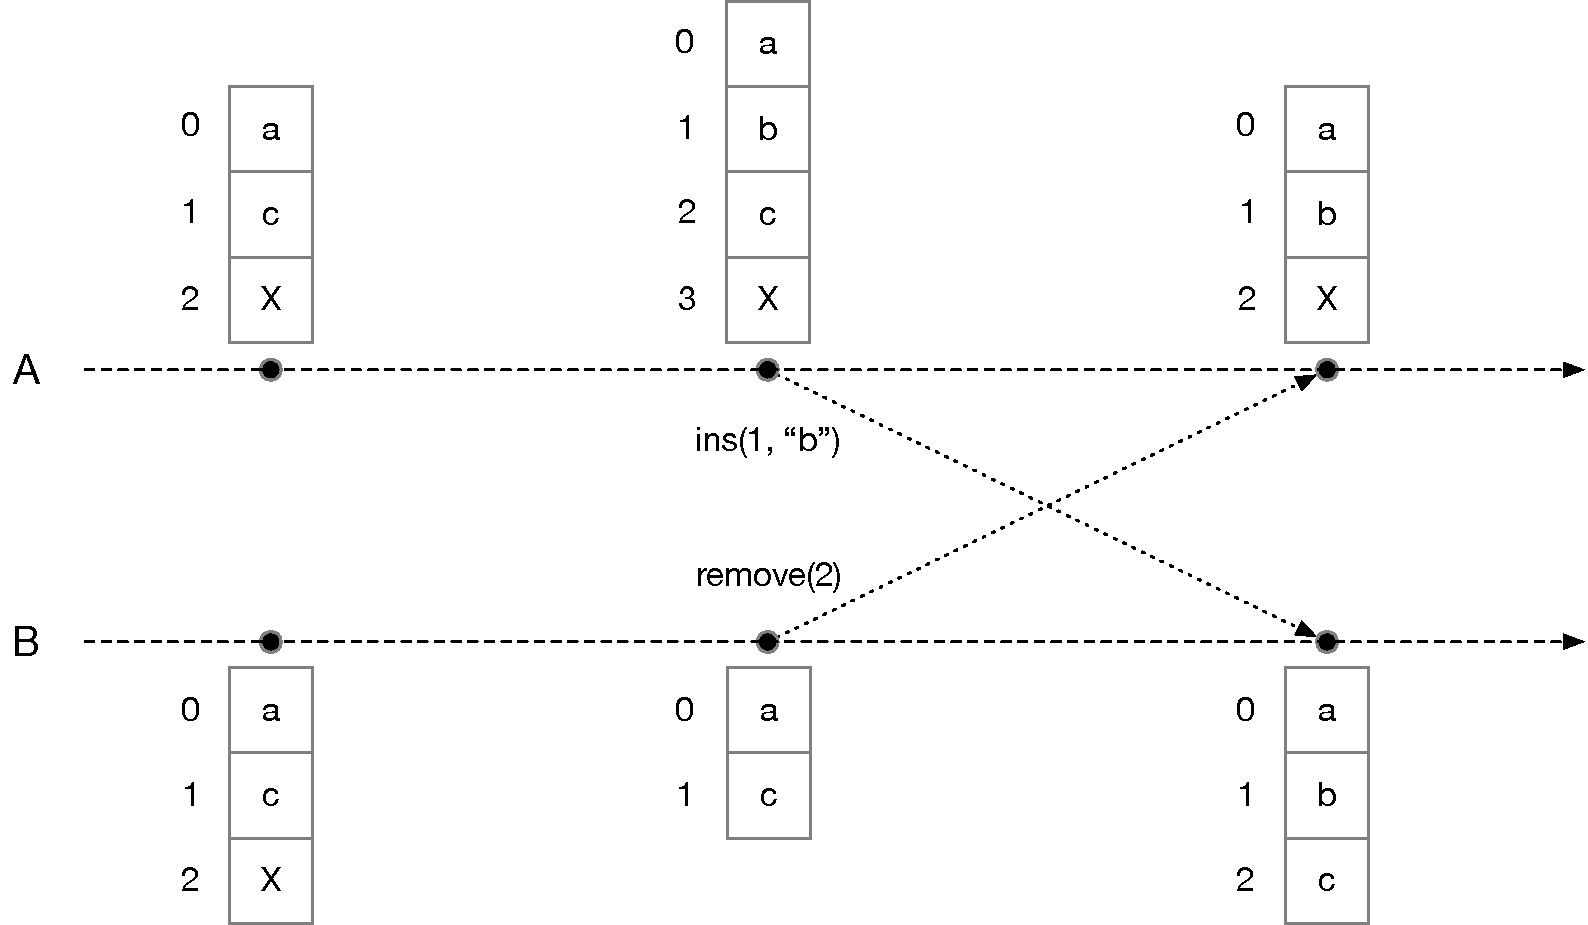
\includegraphics[width=0.75\textwidth]{img/index-based-seq.pdf}
    \caption{Example of concurrent operations on an index-based sequence resulting into an inconsistency}
    \label{fig:basic-seq-divergence}
\end{figure}

This issue is a well-know problem in the domain of collaborative editing and has been an area of research for many years.
\mnnote{TODO: Ajouter des références à des papiers sur OT}
These works eventually led to new specifications of the \emph{Sequence} belonging to a new family of data types: \acfp{CRDT}. \mnnote{TODO: Ajouter référence à WOOT}

\subsection{\acfp{CRDT}}

\acfp{CRDT} \cite{shapiro:inria-00555588, shapiro_2011_crdt} are new specifications of \acp{ADT}, such as the \emph{Set} or the \emph{Sequence}.
Contrary to traditional specifications, \acp{CRDT} are designed to support natively concurrent updates.
To this end, these data types embed directly into their specification a conflict resolution mechanism.
These specifications can be followed to implement optimistically replicated data structures which ensure \acf{SEC} \cite{shapiro_2011_crdt}.

\begin{definition}[Strong Eventual Consistency]\label{def:sec}
\acf{SEC} is a consistency model which guarantees that any two nodes of the distributed system observing the same set of updates reach equivalent states, without requiring any further communications than the ones needed to broadcast the updates.
\end{definition}

These data structures are particularly suited to build highly-available large-scale distributed systems in which nodes share and update data without any coordination.

For a given \ac{ADT}, several specifications of \acp{CRDT} can be proposed.
They can be classified into three categories: State-based \acp{CRDT}, Operation-based \acp{CRDT} and Delta-based \acp{CRDT}.
State-based \acp{CRDT} are often more complex data structures than their Operation-based counterparts, but make no assumptions on the reliability of the message-passing layer.
Operation-based \acp{CRDT} are thus simpler but usually rely on a message-passing layer ensuring the exactly-once causally-ordered delivery of updates.
The third category, the Delta-based \acp{CRDT} one, was more recently proposed and draws out the best from both worlds.

To solve conflicts deterministically and ensure the convergence of all nodes, \acp{CRDT} relies on additional metadata.
In the context of Sequence \acp{CRDT}, two different approaches were proposed, each trying to minimize the overhead introduced.
The first one affixes constant-sized identifiers to each value in the sequence and uses them to represent the sequence as a linked list.
The downside of this approach is an evergrowing overhead, as it needs to keep removed values to deal with potential concurrent updates, effectively turning them into tombstones.
The second one avoids the need of tombstones by instead attaching densely-ordered identifiers to values.
It is then able to order values into the sequence by comparing their respective identifiers.
However this approach also suffers from an increasing overhead, as the size of such densely-ordered identifiers is variable and grows over time.

In this paper, we focus on Densely-identified Operation-based Sequence \acp{CRDT} and propose a renaming mechanism to reduce the metadata overhead introduced by this approach.

\subsection{Logoot}

Logoot \cite{WeissICDCS09} is an Element-wise Densely-identified Operation-based Sequence \ac{CRDT}.
Its key insight is to replace the use of mutable $indexes$ to refer to values into the sequence with immutable $positions$.
As illustrated previously in \autoref{fig:basic-seq-divergence}, in the case of traditional sequences, operations update the sequence and shift values, resulting in inconsistencies when applying several concurrent operations.
By using immutable $positions$ to refer to values, Logoot is able to define a sequence with commutative operations, suited for usages in distributed settings.

When inserting a value into the sequence, the node generates a fitting $position$ and associates it to the value.
These $positions$ fulfill several roles:

\begin{note}
    A $position$ identifies uniquely a value.
\end{note}

\begin{note}
    A $position$ embodies the intended order relation between the value and other values from the sequence.
\end{note}

% \begin{enumerate}
%     \item A $position$ identifies uniquely a value.
%     \item A $position$ embodies the intended order relation between the value and other values from the sequence.
% \end{enumerate}

To perform these roles, $positions$ have to comply to several constraints:

\begin{property}(Global Unicity)\label{prop:global-unicity}
    Nodes should not able to compute the same $position$ concurrently.
\end{property}

\begin{property}(Timeless Unicity)\label{prop:timeless-unicity}
    Nodes should not be able to associate the same $position$ to different values during the lifetime of the sequence.
\end{property}

\begin{property}(Total Order)\label{prop:total-order}
    A total order relation must exist over $positions$ so nodes can order two values given their respective $positions$.
\end{property}

\begin{property}(Dense Set)\label{prop:dense-set}
    Nodes should always be able to generate new $positions$ between two others.
\end{property}

To define $positions$ meeting these properties, Logoot first introduces \emph{LogootTuples} which are specified as in \autoref{spec:logoot-tuple}.
\emph{LogootTuples} are triples made of the following elements:
\begin{itemize}
    \item $priority$: sets the order of this tuple relatively to others, arbitrary picked by the node upon generation
    \item $id_{site}$: refers to the node's identifier, assumed to be unique
    \item $seq_{site}$: refers to the node's logical clock, which increases monotonically with local updates
\end{itemize}

\begin{specification}[LogootTuple]
    \begin{align*}
    &T: \mathsf{LogootTuple} \cdot \spectuple{T}\\
    &T \defeq \tuple{\mathbb{N}, \mathbb{I}, \mathbb{N}}\\
    &\fnspec{constructor}{\mathbb{N} \times \mathbb{I} \times \mathbb{N} \to T}{Returns a LogootTuple made of the given $priority$, $id_{site}$ and $seq_{site}$}\\
    &\queries{priority, peer, seq}\\
    &\commands{}\\
    &\fnspec{priority}{T \to \mathbb{N}}{Returns the $priority$ of the given tuple}\\
    &\fnspec{peer}{T \to \mathbb{I}}{Returns the $id_{site}$ of the given tuple}\\
    &\fnspec{seq}{T \to \mathbb{N}}{Returns the $seq_{site}$ of the given tuple}
    \end{align*}
    \label{spec:logoot-tuple}
\end{specification}

Based on this building block, Logoot defines positions as sequences of \emph{LogootTuples}, as shown in \autoref{spec:logoot-pos}.

\begin{specification}[LogootPos]
    \begin{align*}
    &P: \mathsf{LogootPos} \cdot \spectuple{P}\\
    &T: \mathsf{LogootTuple}\\
    &P \defeq \mathlist{t}{T}\\
    &\fnspec{constructor}{\mathlist{t}{T} \to P}{Returns a LogootPos made of the given tuples}\\
    &\queries{length, get, lastTuple, peer, seq, uid}\\
    &\commands{}\\
    &\fnspec{length}{P \to \mathbb{N}}{Returns the number of tuples composing the position}\\
    &\fnspec{get}{\set{p \in P} \times \set{n \inbb{N} \ssep n < length(p)} \to T}{Returns the n-th tuple of the given position}\\
    &\fnspec{lastTuple}{P \to T}{Returns the last tuple of the given position}\\
    &\fnspec{peer}{P \to \mathbb{I}}{Returns the $id_{site}$ of the last tuple of the given position}\\
    &\fnspec{seq}{P \to \mathbb{N}}{Returns the $seq_{site}$ of the last tuple of the given position}\\
    &\fnspec{uid}{P \to \tuple{\mathbb{I}, \mathbb{N}}}{Returns the unique id of the given position}
    \end{align*}
    \label{spec:logoot-pos}
\end{specification}

It allows positions to meet all the required constraints:
\begin{note}
    Given a position $p$, the couple $\tuple{peer(p), seq(p)}$ is globally and timelessly unique as:
    \begin{itemize}
        \item No other node can generate a position using the same $id_{site}$ as it is unique.
        \item No other position can be generated by the same node using the same $seq_{site}$ as it is increasing monotonically with local updates.
    \end{itemize}
\end{note}

\begin{note}
    A dense total order can be created over positions by:
    \begin{itemize}
        \item Comparing theirs tuples using the lexicographical order.
        \item Defining a special tuple, $minTuple$ such that $\forall t \in LogootTuple \cdot minTuple < t$.
        Given two positions $p1, p2$ such as $p1 < p2$, it allows any node to generate a new position $p3$ such as $p1 < p3 < p2$ by reusing the tuples of $p1$, appending $minTuple$ as many times as required and finally appending a tuple of its own creation.
    \end{itemize}
\end{note}

Relying on these positions, Logoot proposes a new specification corresponding to a replicable sequence, described in \autoref{spec:logoot-seq}.

\begin{specification}[LogootSeq]
    \begin{align*}
    &\forall V: \mathsf{Value} \ \forall S: \mathsf{LogootSeq} \tuple{V} \cdot \spectuple{S}\\
    &P: LogootPos\\
    &S \defeq \set{\tuple{p \in \mathsf{P}, v \in \mathsf{V}}_i}_{i \inbb{N}}\\
    &\fnspec{constructor}{\left( \right) \to S}{Generates and returns an empty Logoot sequence}\\
    &\queries{length, getPos, generatePos}\\
    &\commands{insert, remove}\\
    &\fnspec{length}{S \to \mathbb{N}}{Returns the number of values contained in the sequence}\\
    &\fnspec{getPos}{\set{s \in S} \times \set{n \inbb{N} \ssep n < length(S)} \to P}{Returns ...}\\
    &\fnspec{generatePos}{\mathbb{I} \times \mathbb{N} \times \set{s \in S} \times \set{n \inbb{N} \ssep n < length(S)} \to P}{Returns ...}\\
    &\fnspec{insert}{S \times P \times V \to S}{Inserts the given value into the sequence using its position and returns...}\\
    &\fnspec{remove}{S \times P \to S}{Removes the value from the sequence attached to the given position and returns...}
    \end{align*}
    \label{spec:logoot-seq}
\end{specification}

Using this data type, we can replay the previous scenario while this time ensuring the correctness and convergence of the final states as illustrated in \autoref{fig:logoot-seq-convergence}.

In this scenario, node A wants to insert the value "b" between the values "a" and "c".
To this end, it generates and attaches to "b" a position greater than the position of "a", but lesser than the position of "c".
As there is plenty of room between these two positions, node A is able to generate a position of the same size embodying the intended order.
It that was not the case, node A would have to generate a position by reusing the tuple of "a" and appending to it its own tuple, resulting in a longer position.

Meanwhile, node B wants to remove the value "x" from the sequence.
To do so, it uses the position attached to this value which identifies it uniquely.

\mnnote{TODO: Trouver comment conclure cet exemple}

\begin{figure}
    \centering
        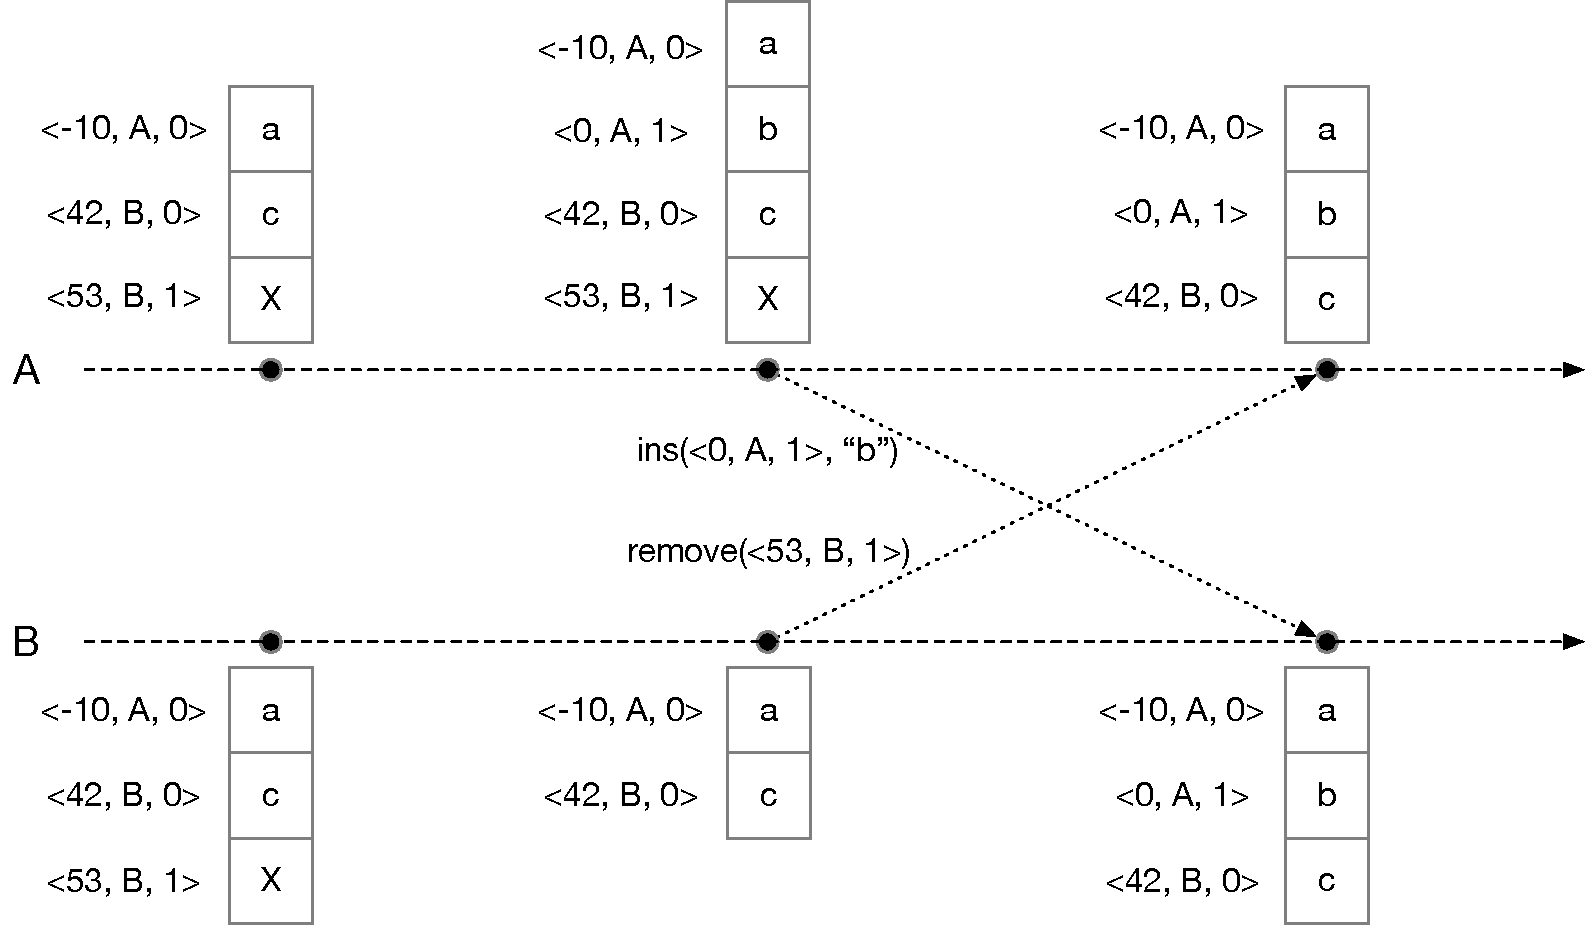
\includegraphics[width=0.75\textwidth]{img/pos-based-seq.pdf}
    \caption{The previous scenario fixed using Logoot positions instead of indexes}
    \label{fig:logoot-seq-convergence}
\end{figure}

\mnnote{TODO: Changer la figure pour utiliser des naturels comme priority, histoire d'être cohérent avec la spécification}

\subsection{LogootSplit}

LogootSplit \cite{AndreCollaborateCom2013} is a Block-wise Densely-identified Operation-based Sequence \ac{CRDT}.
Proposed by \textcite{AndreCollaborateCom2013}, its goal is to improve further the efficiency of the replicated sequence.

Indeed, it is expensive to generate and associate a new position to each value of the sequence.
To reduce the metadata overhead, the authors propose to aggregate dynamically values into blocks.
By regrouping values into blocks, LogootSplit can assign logically a position to each value, while effectively storing only the position of the first value of each block.
This shifts the cause of metadata growth from the number of values to the number of blocks.
As a block can contains an arbitrary number of values, it can lead to a significant increase of the efficiency of the data structure.

To achieve this, LogootSplit adds a new component to the tuples composing its positions, the $offset$.
This component allows to specify the offset of a value into a block.
According to this change, LogootSplit redefines the tuples that it uses as well as the positions, as shown respectively in \autoref{spec:logootsplit-tuple} and \autoref{spec:logootsplit-pos}.

\mnnote{J'aurai bien aimé avoir une abstraction unique pour les Tuples et Positions de Logoot et LogootSplit plutôt que de les redéfinir ici, mais je n'ai pas réussi à la formaliser pour le moment.}

\begin{specification}[LogootSplitTuple]
    \begin{align*}
    &T: \mathsf{LogootSplitTuple} \cdot \spectuple{T}\\
    &T \defeq \tuple{\mathbb{N}, \mathbb{I}, \mathbb{N}, \mathbb{N}}\\
    &\fnspec{constructor}{\mathbb{N} \times \mathbb{I} \times \mathbb{N} \times \mathbb{N} \to T}{Returns a LogootSplitTuple made of the given $priority$, $id_{site}$, $seq_{site}$ and $offset$}\\
    &\queries{priority, peer, seq, offset}\\
    &\commands{}\\
    &\fnspec{priority}{T \to \mathbb{N}}{Returns the $priority$ of the given tuple}\\
    &\fnspec{peer}{T \to \mathbb{I}}{Returns the $id_{site}$ of the given tuple}\\
    &\fnspec{seq}{T \to \mathbb{N}}{Returns the $seq_{site}$ of the given tuple}\\
    &\fnspec{offset}{T \to \mathbb{N}}{Returns the $offset$ of the given tuple}
    \end{align*}
    \label{spec:logootsplit-tuple}
\end{specification}

\begin{specification}[LogootSplitPos]
    \begin{align*}
    &P: \mathsf{LogootSplitPos} \cdot \spectuple{P}\\
    &T: \mathsf{LogootSplitTuple}\\
    &P \defeq \mathlist{t}{T}\\
    &\fnspec{constructor}{\mathlist{t}{T} \to P}{Returns a LogootSplitPos made of the given tuples}\\
    &\queries{length, get, lastTuple, peer, seq, offset, uid}\\
    &\commands{fromBase, concat, truncate}\\
    &\fnspec{length}{P \to \mathbb{N}}{Returns the number of tuples composing the position}\\
    &\fnspec{get}{\set{p \in P} \times \set{n \inbb{N} \ssep n < length(p)} \to T}{Returns the n-th tuple of the given position}\\
    &\fnspec{lastTuple}{P \to T}{Returns the last tuple of the given position}\\
    &\fnspec{peer}{P \to \mathbb{I}}{Returns the $id_{site}$ of the last tuple of the given position}\\
    &\fnspec{seq}{P \to \mathbb{N}}{Returns the $seq_{site}$ of the last tuple of the given position}\\
    &\fnspec{offset}{P \to \mathbb{N}}{Returns the $offset$ of the last tuple of the given position}\\
    &\fnspec{uid}{P \to \tuple{\mathbb{I}, \mathbb{N}, \mathbb{N}}}{Returns the unique id of the given position}\\
    &\fnspec{fromBase}{P \times \mathbb{N} \to P}{Returns a new position made by copying the given position and replacing its offset...}\\
    &\fnspec{concat}{P \times P \to P}{Returns a new position made by concatenating tuples from both given positions}\\
    &\fnspec{truncate}{P \times \mathbb{N} \to P \times P}{Returns a new position made by concatenating tuples from both given positions}
    \end{align*}
    \label{spec:logootsplit-pos}
\end{specification}

Based on its specification of positions, LogootSplit defines the aggregability of positions as follows:

\begin{definition}[Base of a Position]
    The base of a position corresponds to the position deprived of the offset of its last tuple.
\end{definition}

\begin{definition}[Positions Aggregability]
    Two positions are aggregable into a block if they share the same base and if their respective offsets are consecutives.
    It implies that a given block can contain only values inserted by the same node, as the positions have to share the same base thus the same peer.
\end{definition}

\mnnote{FIXME: je ne savais pas où insérer l'highlight sur le fait que les valeurs d'un bloc doivent avoir été insérées par le même noeud donc je l'ai mis dans la définition. À bouger?}

This rule to aggregate positions into blocks results into their following specification.
A block is composed of a position corresponding to the position of its first value, and of the offset of its last value.
LogootSplit can then compute the position of each value of the block by replacing the offset of the first position of the block by the offset of the value.
When inserting a new value into the sequence, LogootSplit first seeks to append or to prepend it respectively to the preceding block or to the succeeding one.
If it is not possible, LogootSplit generates and inserts a new block at the intended place.
To ensure that the positions comply with \autoref{prop:timeless-unicity}, LogootSplit keeps track of the used offsets per block to not reassign the same position to different values.

\begin{specification}[LogootSplitBlock]
    \begin{align*}
    &B: \mathsf{LogootSplitBlock} \cdot \spectuple{B}\\
    &P: \mathsf{LogootSplitPos}\\
    &B \defeq \tuple{\set{p \in P}, \set{n \inbb{N} \ssep offset(p) \leq n}}\\
    &\fnspec{constructor}{P \times \mathbb{N} \to I}{Returns a LogootSplitBlock...}\\
    &\queries{length, posBegin, posEnd, begin, end, peer, seq, uid}\\
    &\commands{}\\
    &\fnspec{length}{B \to \mathbb{N}}{Returns the number of values of the block}\\
    &\fnspec{posBegin}{B \to P}{Returns the first position of the block}\\
    &\fnspec{posEnd}{B \to P}{Returns the last position of the block}\\
    &\fnspec{begin}{B \to \mathbb{N}}{Returns the offset of posBegin}\\
    &\fnspec{end}{B \to \mathbb{N}}{Returns the offset of posEnd}\\
    &\fnspec{peer}{B \to \mathbb{I}}{Returns the peer of the positions of the given block}\\
    &\fnspec{seq}{B \to \mathbb{N}}{Returns the sequence number of the positions of the given block}\\
    &\fnspec{uid}{B \to \tuple{\mathbb{I}, \mathbb{N}}}{Returns the unique id of the given block}
    \end{align*}
    \label{spec:logootsplit-block}
\end{specification}

It is interesting to notice that, in the context of LogootSplit:
\begin{itemize}
    \item Given a position $p$, the triple $\tuple{peer(p), seq(p), offset(p)}$ identifies uniquely this position.
    \item Given a block $b$, the couple $\tuple{peer(b), seq(b)}$ identifies uniquely the base of its positions.
    \item Given a block $b$, the quadruple $\tuple{peer(b), seq(b), begin(b), end(b)}$ identifies uniquely this block.
\end{itemize}

LogootSplit proposes a new specification of the replicated sequence illustrated in \autoref{spec:logootsplit-seq}, supporting string-wise operations. An example of its behavior is shown in \autoref{fig:logootsplit-example}.

\begin{specification}[LogootSplitSeq]
    \begin{align*}
    &\forall V: \mathsf{Value} \ \forall S: \mathsf{LogootSplitSeq} \tuple{V} \cdot \spectuple{S}\\
    &P: LogootSplitPos\\
    &B: LogootSplitBlock\\
    &S \defeq \set{\tuple{b \in \mathsf{B}, \set{v_j \in \mathsf{V}}_{j \inbb {N}}}_i}_{i \inbb{N}}\\
    &\fnspec{constructor}{\left( \right) \to S}{Generates and returns an empty LogootSplit sequence}\\
    &\queries{length, getBlocks, generatePos}\\
    &\commands{insert, remove}\\
    &\fnspec{length}{S \to \mathbb{N}}{Returns the number of values contained in the sequence}\\
    &\fnspec{getBlocks}{\set{s \in S} \times \set{n_1 \inbb{N} \ssep n_1 < length(S)} \times \set{n_2 \inbb{N} \ssep n_1 \leq n_2 < length(S))} \to \mathlist{b}{B}}{...}\\
    &\fnspec{generatePos}{\mathbb{I} \times \mathbb{N} \times \set{s \in S} \times \set{n \inbb{N} \ssep n < length(S)} \to P}{Returns ...}\\
    &\fnspec{insert}{S \times P \times \mathlist{v}{V} \to S}{Inserts the given values into the sequence using its position and returns...}\\
    &\fnspec{remove}{S \times \mathlist{b}{B} \to S}{Removes the values from the sequence attached to the given position...}
    \end{align*}
    \label{spec:logootsplit-seq}
\end{specification}

\begin{figure}
    \centering
        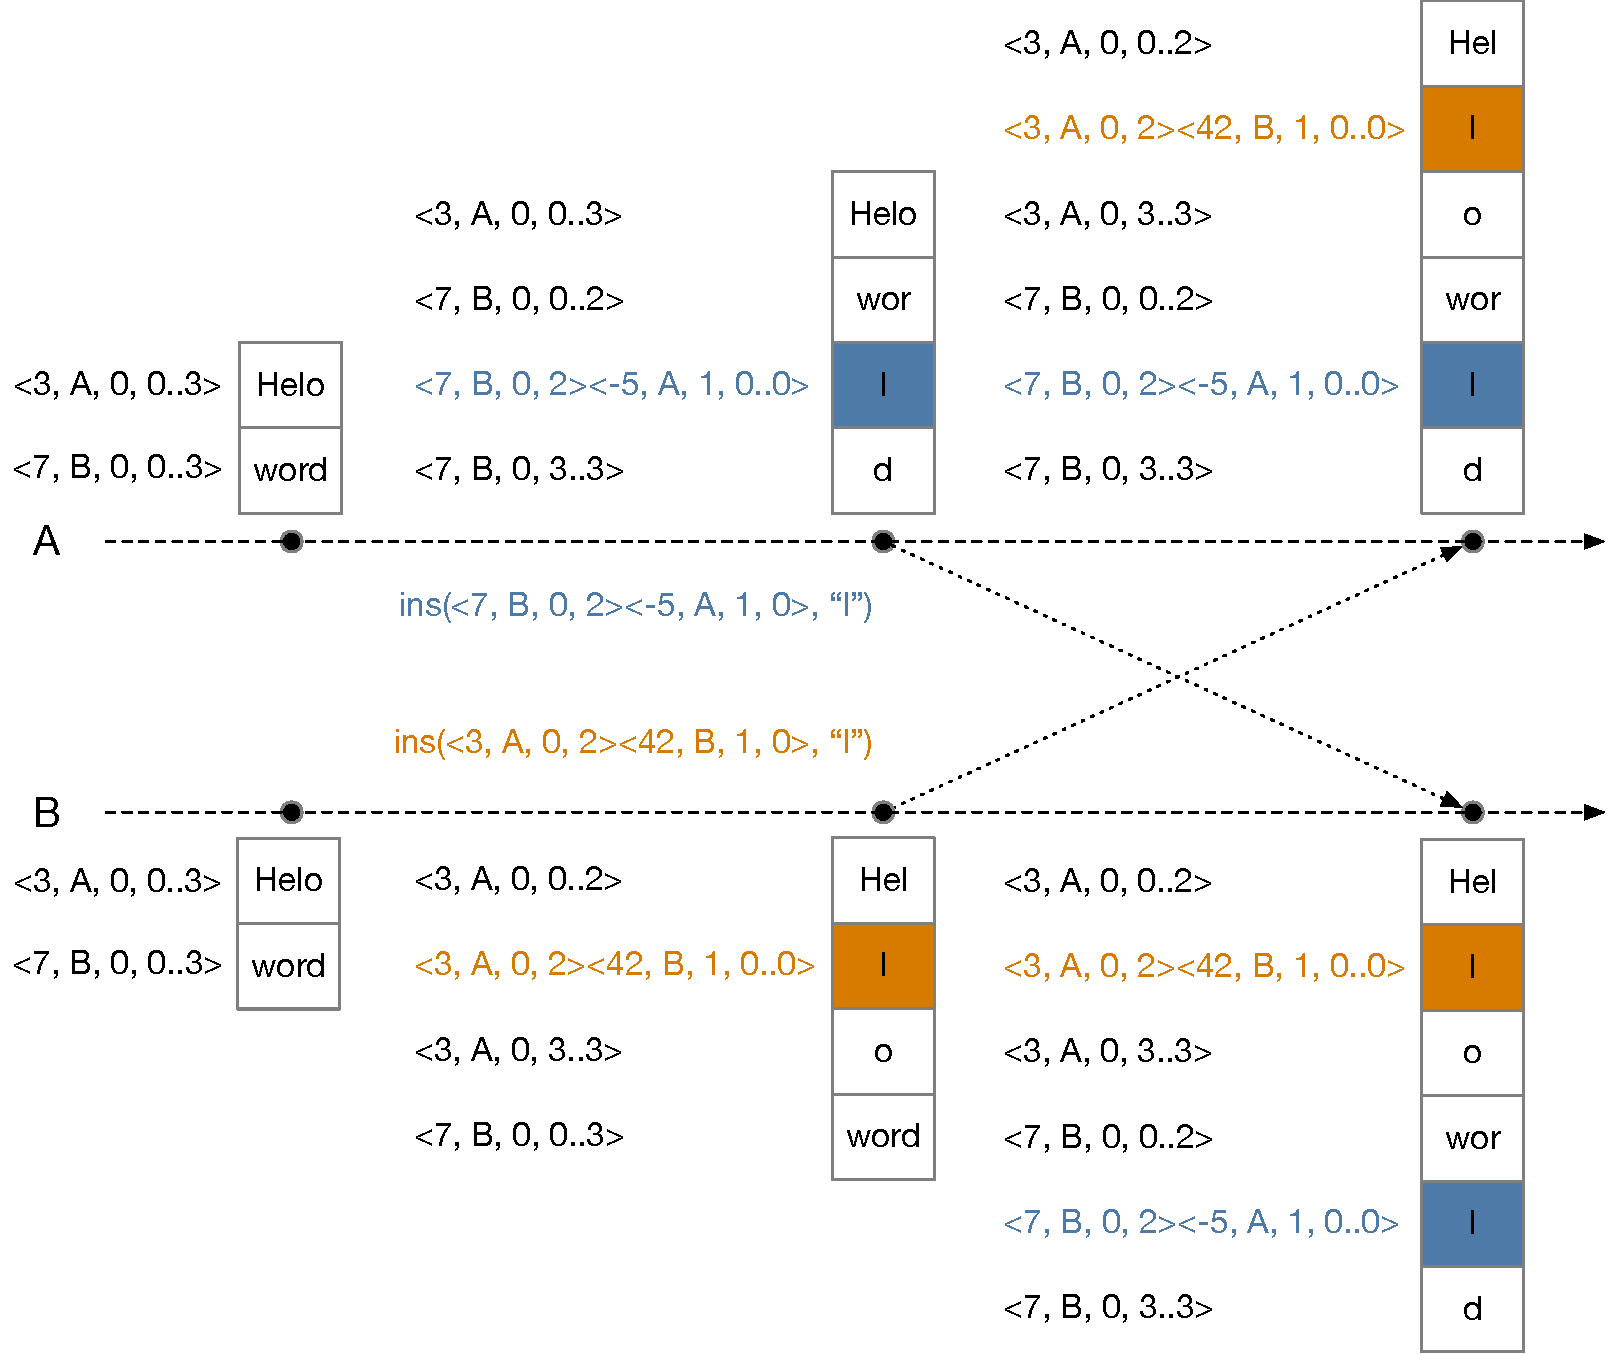
\includegraphics[width=0.6\textwidth]{img/logootsplit-seq.pdf}
    \caption{An example of replicated sequence using LogootSplit}
    \label{fig:logootsplit-example}
\end{figure}

\mnnote{TODO: Finalement, j'aurai tendance à fusionner les sections sur Logoot et LogootSplit pour ne garder que LogootSplit. Dans un premier temps, je peux introduire la notion de position en ne tenant pas compte de offset (ça m'embête juste de mettre l'exemple \autoref{fig:logoot-seq-convergence}, réadapté pour LogootSplit, sans avoir mis la spécification de la séquence au préalable). Puis je peux motiver le fait de regrouper les valeurs par blocs pour réduire l'overhead, expliquer le rôle de offset et remettre l'exemple \autoref{fig:logootsplit-example}.}

\subsection{Limits}

As shown previously, the size of positions in Densely-identified Sequence \acp{CRDT} is not bounded in order to comply with the dense set constraint (\autoref{prop:dense-set}).
As more values are added to the sequence, the size of new positions grows to be able represent the intended order between values.
However, this growth impacts negatively the performances of the data structure on several aspects.
Since positions attached to values become longer, the memory overhead of the data structure increases accordingly.
This also results in an increase of the bandwidth consumption as nodes have to broadcast positions to others.

Additionally, as the lifetime of the replicated sequence increases, the number of blocks composing it grows as well.
Because of the constraints on the generation of positions and their aggregability, it is not always possible to append or prepend new values to existing blocks.
This results in the addition of new blocks to the sequence.
Since no mechanism to merge blocks a posteriori is provided, the resulting sequence ends up being fragmented into many blocks.
The efficiency of the data structure decreases as each block introduces its own metadata overhead.

\mnnote{TODO: Illustrer l'augmentation de l'overhead avec un graphe.}

\mnnote{TODO: Ajouter aussi des métriques sur l'évolution de la taille des identifiants, du nombre de blocs ?}

\mnnote{TODO: Ajouter une phrase sur le fait qu'on se retrouve avec une séquence répliquée jusqu'à 100x plus lourde que la séquence équivalente non-répliquée. Cette mesure pose cependant un problème : elle repose sur notre implémentation actuelle de LogootSplit qui ne réutilise pas la même instance d'un tuple partagé par plusieurs identifiants. L'utilisation d'un pattern Multiton résoudrait ce problème et limiterait le poids de la structure de données et donc le résultat des mesures (mais ajouterait une complexité supplémentaire qui serait de traquer quand on peut GC un tuple).}

It is thus necessary to either propose a more efficient specification of the replicated list, with a reduced growth of the overhead
or to provide a mechanism allowing to reset the overhead of the data structure at times.
In this paper, we present a work corresponding to the later approach.

\section{Overview}

We propose a new Densely-identified Operation-based Sequence \ac{CRDT}: \emph{RenamableLogootSplit}.

To address the limitations of LogootSplit, we embed in this data structure a renaming mechanism.
The purpose of this mechanism is to reassign shorter positions to values in such a manner that we are then able to aggregate them into one unique block.
This allows to reduce the bandwidth used to broadcast future updates as well as the metadata of the whole sequence.
However, as the goal is to reduce LogootSplit's evergrowing memory overhead and bandwidth consumption, we have to design the renaming mechanism while minimizing its own footprint.

\subsection{System Model}

The system is composed of a dynamic set of nodes, as nodes join and leave dynamically the collaboration during its lifetime.
Each node has a unique identifier from a set $\mathbb{I}$.
The nodes collaborate to build and maintain a sequence using RenamableLogootSplit.
Each node owns a copy of the sequence and edit it without any kind of coordination with others.

However, the network is unreliable.
Messages can be lost, re-ordered or delivered multiple times.
The network is also vulnerable to partitions, which split nodes into disjoined subgroups.
To overcome the failures of the network, nodes rely on a message-passing layer.
As RenamableLogootSplit is built on top of LogootSplit, it shares the same requirements for the operation delivery.
This layer is thus used to deliver messages to the application exactly-once.
The layer also ensures that \emph{remove} operations are delivered after corresponding \emph{insert} operations.
Nodes use an anti-entropy mechanism to synchronise in a pairwise manner, by detecting and re-exchanging lost operations.

\subsection{Specification}

We introduce a new operation, the \emph{rename} one.
Nodes use this operation to define and share a common context between them.
Each node use this context to map positions of their current sequence to new ones.
This mapping is perform using a new function introduced : $renamePos$.

However, the mapping must be done while preserving the safety properties of the system.
These properties are the following:

\begin{property}(Well-formed Sequence)
    The sequence must be well-formed.
    We define a sequence as well-formed if it meets the following conditions:
    \begin{itemize}[noitemsep]
        \item[~]
        \begin{subproperty}(Unicity Preservation)
            Each position must be unique.
            Thus, for a given \emph{rename} operation, each position should be mapped to a distinct new position.
        \end{subproperty}
        \item[~]
        \begin{subproperty}(Order Preservation)
            The sequence must be sorted with regards to the positions.
            Therefore, the existing order between initial positions must be preserved by the mapping.
        \end{subproperty}
    \end{itemize}
\end{property}

\begin{property}(\acf{SEC})
    All nodes which received the same set of operations must converge without any further coordination.
    To ensure this property, operations must be designed to comply with the following constraints:
    \begin{itemize}[noitemsep]
        \item[~]
        \begin{subproperty}(Deterministic Operations)
            Operations are applied by each node without any coordination.
            To ensure that each node reaches eventually the same state, operations must always produce the same output.
        \end{subproperty}
        \item[~]
        \begin{subproperty}(Commutative Concurrent Operations)
            Concurrent operations may be delivered in different orders at each node.
            In order to ensure the convergence of nodes, the order of application of a set of concurrent operations should not have any impact on the resulting state.
        \end{subproperty}
    \end{itemize}
\end{property}

\subsection{Proposition}
\label{sec:proposition}

\mnnote{TODO: Introduire l'exemple}

In this example, two nodes, A and B, own a copy of the same replicated sequence.
Initially, their respective states are equivalent.
Node A issues a \emph{rename} operation: new positions of minimal size are reassigned to each value of the sequence.
These new positions are picked in such a way that make it possible to aggregate all values into one block.
Concurrently, node B inserts a new value into the sequence.
To this end, the node computes and attaches a position to the value.
Both operations are then broadcasted.

Upon reception of the \emph{insert} operation, node A does not apply it as it is.
Indeed, as positions of other values have been modified, inserting the new value at its given position would result in an inconsistency: the breach of the intended order.
Therefore, it is necessary to rename this position and thus to transform the operation before applying it.
Once a fitting new position has been computed, the value can be safely inserted into the sequence.
When node B received the \emph{rename} operation, it applies the renaming on each position of its current sequence to obtain the new state.

\begin{figure}
    \centering
    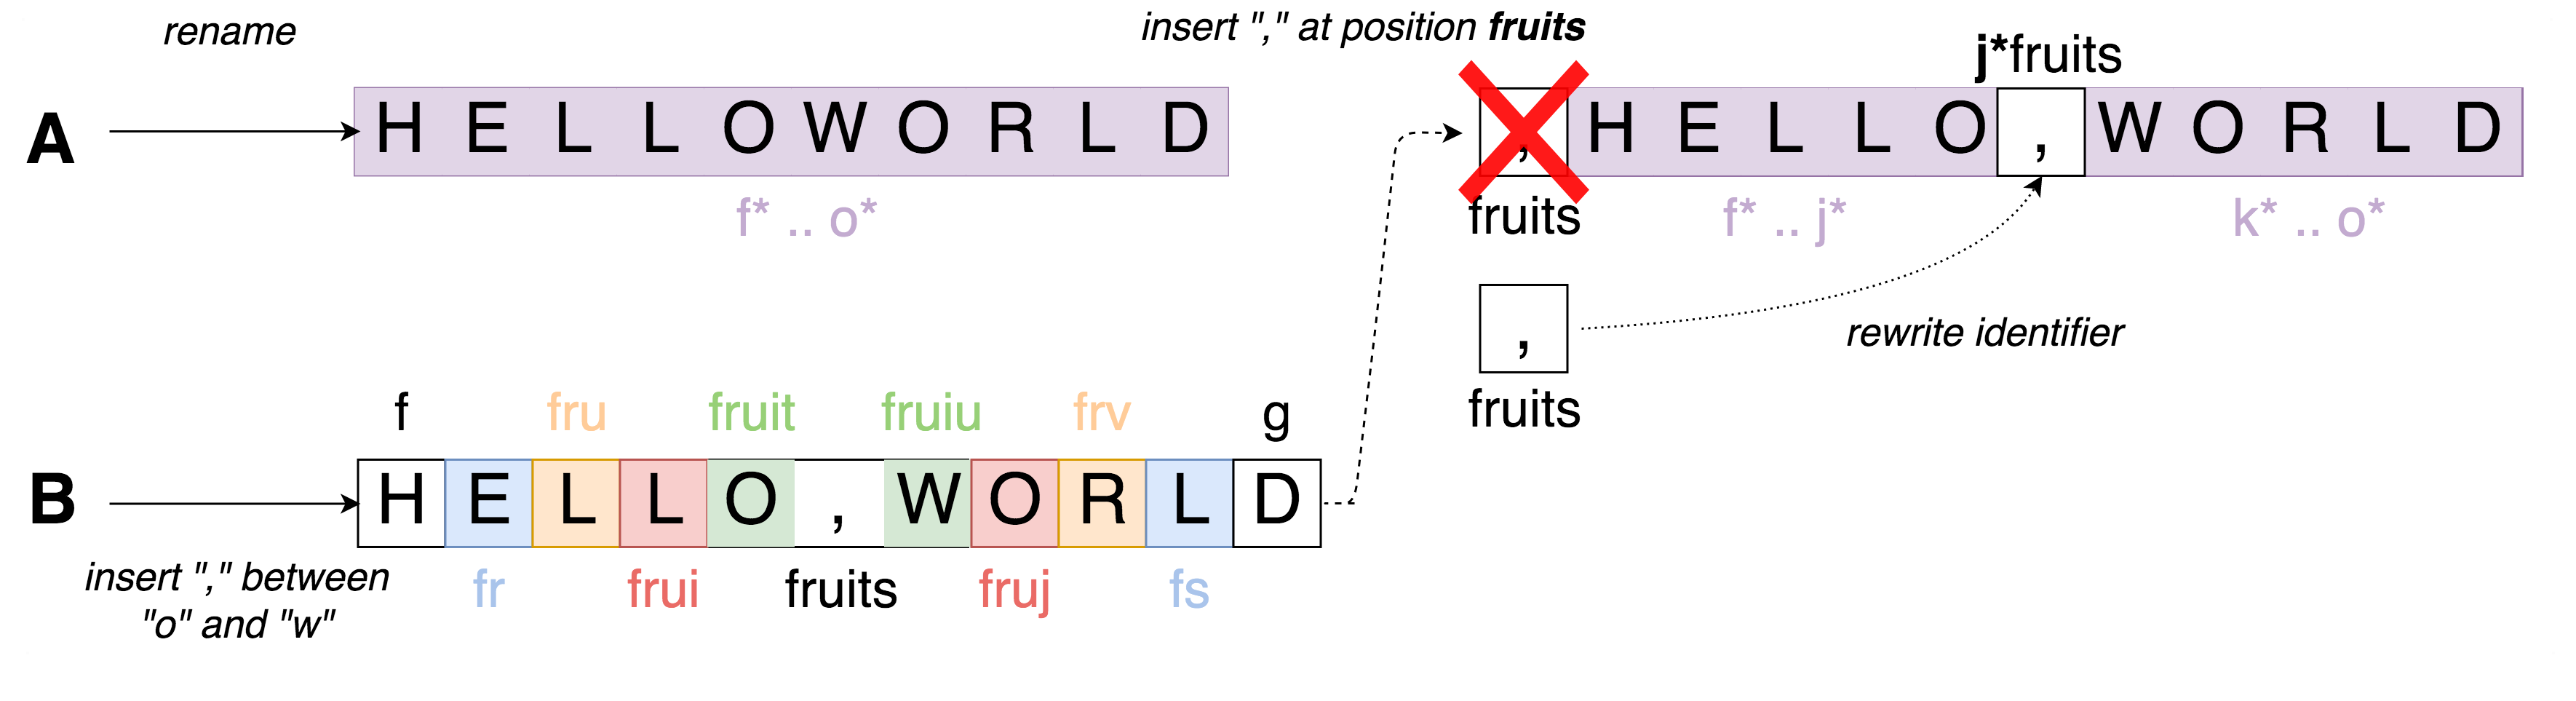
\includegraphics[width=0.75\textwidth]{img/example-renaming.png}
    \caption{Concurrent \emph{rename} and \emph{insert} operations}
    \label{fig:example-renaming}
\end{figure}

\mnnote{TODO: Reprendre \autoref{fig:example-renaming} et unifier son formalisme et style avec le reste des figures.}
In the next sections, we describe how we designed and implemented such renaming mechanism.
For simplicity purposes, we present first RenamableLogootSplit under the assumption that no concurrent renamings can take place.
This allows us to illustrate the process of renaming the sequence and how to design it to be commutative with \emph{insert} and \emph{remove} operations.
We then present the complete version of RenamableLogootSplit, with the additional components required to deal with concurrent renamings.

\section{Renaming without any concurrent \emph{rename} operation}

\subsection{\emph{Epoch-based} mechanism}

A renaming can be seen as a change of frame of reference, applied to positions.
Positions come from different frames according to if \emph{rename} operations occurred between their generation.
As illustrated in \autoref{sec:proposition}, comparing positions from different frames and taking decision on this result would lead to inconsistencies.
It is thus necessary to define the frame of reference in which a given position is valid and to add information to the system to model it.

To this end, we introduce the notion of \emph{epochs}.
The sequence is first assigned a default epoch : the \emph{origin} one.
As the default epoch \emph{origin} does not belong to any actual node, we define and use a specific $id_{site}$ noted as $\bot_{\mathbb{I}}$ for this particular case.
Upon the delivery of a \emph{rename} operation, nodes update the current epoch of their sequence with a newly generated one.
We generate this new epoch using $id_{site}$ and $seq_{site}$ of the node which issued the operation to make it unique.
We will then have to embed this data into the \emph{rename} operation.

Thus, we specify epochs as follows:

\begin{specification}[Epoch]
    \begin{align*}
    &E: \mathsf{Epoch} \cdot \spectuple{E}\\
    &E \defeq \set{origin, \tuple{n, \mathbb{I}} \ssep n \in \mathbb{N^*}}\\
    &origin = \tuple{0, \bot_{\mathbb{I}}}\\
    &\fnspec{constructor}{\mathbb{I} \times \mathbb{N} \to E}{Returns an Epoch made of the given $id_{site}$ and $seq_{site}$}\\
    &\queries{peer, seq, epochId}\\
    &\commands{}\\
    &\fnspec{peer}{E \to \mathbb{I}}{TODO}\\
    &\fnspec{seq}{E \to \mathbb{N}}{TODO}\\
    &\fnspec{epochId}{E \to \tuple{\mathbb{I}, \mathbb{N}}}{TODO}
    \end{align*}
    \label{spec:epoch}
\end{specification}

We tag operations with the current epoch at their time of generation to encapsulate their scope of validity.
Upon reception of an operation, nodes first compare the current epoch of their sequence to the epoch embedded in the operation.
If the two epochs match, the operation can be applied at it is.
Otherwise, nodes need to transform the operation beforehand.

As operations are now tied to the concept of epochs, we have to update the existing constraints on their order of delivery.
Delivering operations originating from an epoch unknown to a node would cause issues, as the node would have no clue on how to deal with them.
Thus, we define the new consistency model used by the message-passing layer as follows:

\begin{specification}("Epoch-based + Causal Remove" Consistency Model)
    The message-passing layer delivers operations according to the following constraints:
    \begin{enumerate}
        \item Operations are delivered causally to \emph{rename} operations which introduced their respective epochs.
        \item {remove} operations are delivered after corresponding \emph{insert} operations.
    \end{enumerate}
\end{specification}

\subsection{Generating \emph{rename} operations}

In order to ensure \ac{SEC}, nodes have to apply each operation in a coordination-free manner.
In our case, nodes have to rename any position the same way without coordinating.
However, nodes may observe operations in different orders.
They may not share the same state when applying the \emph{rename} operation.
Then we can not rely on their respective state to take any decision on how to rename a position.
We thus design the \emph{rename} operation to provide and set a common context between nodes.
This common context will be used to rename positions in a deterministic fashion without requiring further communications.

We thus specify \emph{rename} operations as follows:

\begin{specification}[Rename Operation]
    \begin{align*}
    &R: \mathsf{RenameOp} \cdot \spectuple{R}\\
    &R \defeq \tuple{E, \mathbb{I}, \mathbb{N}, \mathlist{b}{B}}\\
    &\fnspec{constructor}{E \times \mathbb{I} \times \mathbb{N} \times \mathlist{b}{B} \to R}{Returns a \emph{rename} operation made of the given $epoch$, $id_{site}$, $seq_{site}$ and $renamedBlocks$}\\
    &\queries{epoch, peer, seq, renamedBlocks}\\
    &\commands{}\\
    &\fnspec{epoch}{R \to E}{TODO}\\
    &\fnspec{peer}{R \to \mathbb{I}}{TODO}\\
    &\fnspec{seq}{R \to \mathbb{N}}{TODO}\\
    &\fnspec{renamedBlocks}{R \to \mathlist{b}{B}}{TODO}
    \end{align*}
    \label{spec:rename}
\end{specification}

However, the metadata overhead per block is not bounded, as blocks rely on positions which are themselves not bounded.
Moreover, the number of blocks grows as the collaboration progresses until a \emph{rename} operation is applied.
Broadcasting \emph{rename} operations may then prove to be expensive.

To adress this issue, we present a mechanism to compress the \emph{rename} operation in \autoref{sec:optimisation-rename-op}.
This mechanism allows to reduce to a fixed amount the metadata per block at the price of additional computations.
Furthermore, we configure nodes to issue a \emph{rename} operation once the number of blocks in the sequence reaches a given treshold.
This effectively limits the number of blocks that \emph{renamedBlocks} may contain.

Combining these two actions thus allow us to bound the size of \emph{rename} operations.

\subsection{Renaming positions}
\label{sec:renameForwardPos}

Thanks to the data embedded in the \emph{rename} operations, nodes are now able to rename positions in a convergent way.
To this end, we define the new function $renameForwardPos$, which rename a given position $pos$ into a new position based on the provided $renamedBlocks$.
Its behavior, which is detailed in algorithm \ref{alg:renameForwardPos}, can be described as follows.

This algorithm distinguishes two cases: if the given position $pos$ is part of the known positions when the \emph{rename} operation was issued, or not.
In the first case, we map the position to one of the position of the resulting block.
In the other case, we generate a new unique position respecting the intended order.

We start by checking in which case we find ourselves.
To this end, we use the function $hasBeenRenamed$.
This function browses $renameBlocks$ to determine if $pos$ is contained in one of the blocks.

If that is the case, we use the function $findIndex$ to retrieve the corresponding index of $pos$ in the sequence.
Using this index, we generate and return the new corresponding position.

Otherwise, it means that $pos$ has been inserted concurrently to the \emph{rename} operation. \mnnote{NOTE: On peut aussi rencontrer cette situation si $pos$ a été supprimée avant (dans le sens happen-before) que l'opération de renommage ne soit générée, mais que le modèle de cohérence utilisé par l'application autorise la livraison du renommage avant celle de la suppression (ce qui va être notre cas). Rentrer à ce niveau de détail?}
We have to transform it to preserve the existing order.
According to the value of $pos$, we apply different strategies to generate its image: $newPos$.

We define $firstPos$ the first position of the first block of $renamedBlocks$ and $lastPos$ the last position of the last block.
We call $newFirstPos$ and $newLastPos$ their respective image regarding $renameForwardPos$.

The first strategy is applied to positions which are included in the interval $]firstPos, lastPos[$.
In that case, we first search $predecessor$, the predecessor of $pos$ in $renamedBlocks$, using the function $findPredecessor$.
Then, we retrieve the index of $predecessor$ thanks to $findIndex$.
Using its index, we can compute the new position corresponding to $predecessor$: $newPredecessor$.
Finally, we generate $newPos$ by concatenating $pos$ to $newPredecessor$.

The second case is for positions such as we have $lastPos < pos < newLastPos$.
To preserve the intended order between positions, we have to generate $newPos$ such as $newLastPos < newPos$.
We achieve it by concatenating $pos$ to $newLastPos$ to obtain $newPos$.

The third case is for positions such as we have $newFirstPos < pos < firstPos$.
In that scenario, we have to generate $newPos$ such as $newPos < newFirstPos$.
To this end, we pick the predecessor of $newFirstPos$, $predecessorOfNewFirstPos$, by decreasing its offset by one.
We then generate $newPos$ by concatenating $pos$ to $predecessorOfNewFirstPos$.

Finally, in all other cases, we return $pos$ unchanged.
Indeed, positions from previous cases are mapped to positions belonging to the interval $]predecessorOfNewFirstPos, successorOfNewLastPos[$.
As all remaining positions are either smaller than $predecessorOfNewFirstPos$ or greater than $successorOfNewLastPos$, we can safely return it without any risk of breaking the existing order.

% Generating $newPos$ by concatenating $pos$ to a prefix allows us to preserve easily the existing order between positions.
% Given two positions $pos$ and $pos'$ inserted concurrently to the \emph{rename} operation, either they have different predecessors in $renamedBlocks$, either they share the same one.
% In the first case, as the new positions corresponding to their respective predecessor will be used as prefixes, the resulting positions $newPos$ and $newPos'$ will be ordered according to them.
% In the second case, since they share the same prefix, the order between $newPos$ and $newPos'$ effectively comes down to the order between $pos$ and $pos'$.
% In both case, we have $newPos$ < $newPos'$.


\begin{algorithm}
    \caption{Rename position}
    \label{alg:renameForwardPos}
    \begin{algorithmic}[1]
    \Function{renameForwardPos}{$pos: P, newId: \mathbb{I}, newSeq: \mathbb{N}, renamedBlocks: \mathlist{b}{B}$}{: $P$}
        \State $firstPos \gets posBegin(renamedBlocks[0])$
        \State $lastPos \gets posEnd(renamedBlocks[renamedBlocks.length - 1]$\\

        \State $newPriority \gets priority(firstPos)$
        \State $newFirstPos \gets new \ P(newPriority, newId, newSeq, 0)$
        \State $newLastPos \gets new \ P(newPriority, newId, newSeq, length)$\\

        \If{$hasBeenRenamed(pos, renamedBlocks)$}
            \State $index \gets findIndex(pos, renamedBlocks)$
            \State \Return $new \ P(newPriority, newId, newSeq, index)$
        \ElsIf{$firstPos < pos$ \textbf{and} $pos < lastPos$}
            \State $predecessor \gets findPredecessor(pos, renamedBlocks)$
            \State $indexOfPredecessor \gets findIndex(predecessor, renamedBlocks)$
            \State $newPredecessor \gets new \ P(newPriority, newId, newSeq, indexOfPredecessor)$
            \State \Return $concat(newPredecessor, pos)$
        \ElsIf{$lastPos < pos$ \textbf{and} $pos < newLastPos$}
            \State \Return $concat(newLastPos, pos)$
        \ElsIf{$newFirstPos < pos$ \textbf{and} $pos < firstPos$}
            \State $predecessorOfNewFirstPos \gets new \ P(newPriority, newId, newSeq, -1)$
            \State \Return $concat(predecessorOfNewFirstPos, pos)$
        \Else
            \State \Return $pos$ \Comment Return the position unchanged as it does not interfere with the renaming
        \EndIf
    \EndFunction
    \end{algorithmic}
\end{algorithm}

\begin{figure}
    \centering
    \includegraphics[width=\textwidth]{img/filler-example-renameforwardpos.JPG}
    \caption{TODO: À refaire sur papier, là on voit rien...}
    \label{fig:example-renameforwardpos}
\end{figure}

% \begin{itemize}
%     \item
%     \begin{itemize}
%         \item If $pos$ was one of the positions belonging to the state when the $renamingMap$ was computed, then its renaming has already been decided and its new value is stored in the $renamingMap$. We just return it.
%         \item If that is not the case, we need to compute the new position corresponding to it in the new frame of reference
%         \item To be able to preserve the existing order between $pos$ and other positions through the renaming, we use different strategies according to the position's value:
%         \begin{itemize}
%             \item We define respectively as $firstPos$ and $lastPos$ the first and last positions contained in the entries of the $renamingMap$, and $newFirstPos$ and $newLastPos$ their images in the new frame of reference.
%             \item If $pos$ is actually outside of the range impacted by the renaming, i.e \\ $pos < min(firstPos, newFirstPos)$ or $max(lastPos, newLastPos) < pos$, we can return it unchanged as it will not conflict with other renamed positions
%             % \item If we have $lastPos < pos < newLastPos$, we rename $pos$ to shift it just after $newLastPos$ by concatenating $pos$ to $newLastPos$.
%             \item If we have $newFirstPos < pos < firstPos$, we rename $pos$ to shift it just before $newFirstPos$ by concatenating $pos$ to the predecessor of $newFirstPos$. The predecessor of $newFirstPos$ is obtained by subtracting 1 to its $offset$ part.
%             \item In the remaining case, it means that we have $firstPos < pos < maxLastPos$. In this case, we look for $predecessorOfPos$, the predecessor of $pos$ among the keys of $renamingMap$. Then, we retrieve the image of this position in the new state, $newPredecessorOfPos$. By concatenating $pos$ to $newPredecessorOfPos$, we are able to generate a new position while preserving the existing order.
%         \end{itemize}
%     \end{itemize}
%     \item The main idea of this approach is to preserve the existing order between positions by concatenating the former positions to given prefixes to form the new positions.
%     \item The greater the original position, the greater the prefix used to compose the new position.
%     \item So, with $p1$ and $p2$ two positions such as $p1 < p2$ and $p1'$ and $p2'$ their respective renamed versions, we have
%     \begin{itemize}
%         \item either $p1'$ and $p2'$ sharing the same prefix. In that case, comparing $p1'$ and $p2'$ effectively comes down to comparing $p1$ and $p2$.
%         \item either the prefix of $p2'$ is greater than the prefix of $p1'$.
%     \end{itemize}
%     \item In both cases, we have $p1' < p2'$.
%     \item \mnnote{NOTE: Ce que je dis au-dessus concerne le cas où on a $firstPos < p1 < p2 < maxLastPos$, mais est vrai aussi pour le cas où on a $newFirstPos < p1 < firstPos < p2$ de façon moins évidente.
%     \\
%     Reste à montrer que l'ordre est conservé dans les cas limites ($p1 < newFirstPos < p2  < firstPos$; $p1 < maxLastPos < p2$).
%     \\
%     Renvoyer à la section validation.}
% \end{itemize}

\subsection{Applying \emph{rename} operation}

Upon the delivery of a \emph{rename} operations, nodes execute the following steps to apply it.

First, they retrieve the newly generated epoch using the $id_{site}$ and $seq_{site}$ embedded in the operation.
They update the current epoch of their state.
Their future operations will then be tagged using this new epoch onward.

Second, using the \emph{renamedBlocks} contained in the operation and the function $renameForwardPos$, nodes rename each position of their current state.
Resulting positions are then aggregated into blocks and a new sequence is built from them, replacing the previous one.

However, nodes may still received operations from previous epochs.
Some of these operations may even be outdated by several \emph{rename} operations.
To apply these operations, nodes will have to transform them beforehand.
Nodes thus need to store the \emph{renamedBlocks} and have to be able to compute the list of epochs separating two others.

To this end, we add a new data structure to the replicated sequence: the \emph{Epoch Store}.
Nodes register into the \emph{Epoch Store} each epoch and the corresponding \emph{renamedBlocks}.
Newly inserted epochs are linked to the previous epoch by a parent-child relationship.
% We use this relationship to define the order relationship between epochs.
% We define an epoch as greater than its ancestors.

\begin{specification}[Epoch Store]
    \begin{align*}
    &ES: \mathsf{EpochStore} \cdot \spectuple{ES}\\
    &ES \defeq \set{\tuple{E, E, \mathlist{b}{B}}}\\
    &\fnspec{constructor}{() \to ES}{Returns an empty Epoch Store}\\
    &\queries{epoch, parentEpoch, renamedBlocks, getPathForwardBetweenEpochs}\\
    &\commands{add}\\
    &\fnspec{epoch}{ES \times \tuple{\mathbb{I}, \mathbb{N}} \to E}{TODO}\\
    &\fnspec{parentEpoch}{ES \times E \to E}{TODO}\\
    &\fnspec{renamedBlocks}{ES \times E \to \mathlist{b}{B}}{TODO}\\
    % &\fnspec{compareEpochs}{ES \times E \times E \to \{ <, >, = \}}{TODO}
    &\fnspec{getPathForwardBetweenEpochs}{ES \times E \times E \to \mathlist{e}{E}}{TODO}\\
    %&\fnspec{getPathForwardBetweenEpochs}{ES \times \{ e_1 \in E \} \times \{ e_2 \in E \ssep e_1 < e_2 \} \to \mathlist{e}{E}}{TODO}\\
    &\fnspec{add}{ES \times \tuple{E, E, \mathlist{b}{B}} \to ES}{TODO}
    \end{align*}
    \label{spec:epoch-store}
\end{specification}

\subsection{Applying \emph{insert} and \emph{remove} operations}

Upon the reception of a \emph{insert} or \emph{remove} operation, nodes first compare their current epoch to the operation's one.
If the two epochs match, then nodes can apply the operation as it is.
Otherwise, it means that one or several \emph{rename} operations were applied locally since this operation has been issued.
Nodes have to transform the operation beforehand to preserve its semantic.

In that case, nodes retrieve the list of these renamings using the \emph{Epoch Store}, the current epoch and the operation's one.
They rename successively the positions of the operation to build the corresponding positions in the new epoch.
Using them, nodes build the new operation and apply it to their state.

% \subsection{Putting it all together}

% \mnnote{
%     TODO: Expliquer qu'on propose un nouveau CRDT, \emph{<insérer un nom ici>} (RenamableLogootSplit?).
%     \\
%     Cette structure de données encapsule une liste répliquée en utilisant LogootSplit, mais maintient aussi l'epoch courante, une map des epochs et les renamingMaps permettant d'avancer d'une epoch à l'autre.
%     \\
%     Dispose des fonctions présentées précédemment, generateRenamingMap() et renameForwardPos().
%     \\
%     Propose la fonction $rename()$ qui retourne la séquence renommée en appliquant $renameForwardPos$ à chaque position de l'état courant.
%     \\
%     Surcharge le traitement des opérations $insert$ et $delete$ pour:
%     \\
%         - Déléguer le traitement de l'opération à l'instance de LogootSplit si l'epoch de génération correspond à l'epoch courante
%         \\
%         - Ou transformer l'opération au préalable à l'aide de renameForwardPos() (potentiellement à travers plusieurs epochs) si les epochs ne correspondent pas.
%         \\
%     Indiquer qu'on a une contrainte supplémentaire pour la livraison des opérations : elles doivent être livrées dans l'ordre causal par rapport à la dernière opération de renommage observée (doit être à la même epoch que celle de génération de l'opération ou à une epoch suivante pour pouvoir appliquer une opération).
% }

\subsection{Garbage collection}

\begin{itemize}
    \item As stated previously, the renaming mechanism generates and stores additional metadata: the epochs and the renamingMaps used to transform concurrent operations against the renaming
    \item However, we do not need to keep this additional metadata forever
    \item Since they are used to handle concurrent operations to the renaming, they are not required anymore once no additional concurrent operation can be issued by a node
    \item i.e. we can safely garbage collect rewriting rules once the corresponding renaming operation is causally stable \cite{10.1007/978-3-662-43352-2_11}
    \item Nodes need thus to keep track of the progress of others to detect when this condition is met
    \item This can be done in a coordination-free manner by exploiting the epochs attached to operations:
    \begin{itemize}
        \item Each node stores a vector of epochs, with one entry for each node
        \item Upon the reception of an operation, the node updates the entry of the sender with the epoch of the operation
        \item As nodes collaborates, epochs in the vector will progress
        \item By retrieving the minimum epoch from the vector, we can identify which epoch has been reached by all nodes
        \item We can then safely garbage collect all previous epochs and corresponding renamingMaps
    \end{itemize}
\end{itemize}

\section{Evaluation}

To validate the proposed renaming mechanism, we performed an experimental evaluation to measure its performances on several aspects:
\begin{enumerate*}
    \item the size of the data structure
    \item the integration time of the \emph{rename} operation
    \item the integration time of \emph{insert} and \emph{remove} operations.
\end{enumerate*} In cases 1 and 3, we use LogootSplit as the baseline data structure to compare results.

Since we were not able to retrieve an existing dataset of traces of realtime collaborative editing sessions, we ran simulations to generate traces to evaluate our data structure.
The simulations depict the following scenario: several authors collaborate in order to write an article.
Initially, they prioritize adding content as everything remains to be done.
Thus they mainly insert elements into the document during this first phase.
A few \emph{remove} operations are still issued to simulate spelling mistakes.
Once the document approaches the critical length, the collaborators switch to the second phase.
From this point, they stop adding new content and focus on revamping existing parts instead.
This is simulated by balancing the ratio between \emph{insert} and \emph{remove} operations.
Each bot has to perform a given number of operations and the collaboration ends once every bot received all operations.
We take snapshots of the document at given steps of the collaboration to follow the evolution of the document.

We ran these simulations with the following experimental settings : we deployed 10 bots as separate Docker containers on a single workstation.
Each container corresponds to a single mono-threaded Node.js process (version 13.1.0) simulating an author.
The bots share and edit collaboratively the document using either LogootSplit or RenamableLogootSplit according to the session.
In both cases, each bot performs an \emph{insert} or a \emph{remove} operation locally every 200 $\pm$ 50ms.
During the first phase, the probabilities for each operation of being an \emph{insert} or a \emph{remove} are respectively of 80\% and 20\%.
Once the document reaches 60k characters (around 15 pages), the probabilities are both set to 50\%.
The generated operation is then broadcast to others using a \ac{P2P} full mesh network.
After issuing an operation, there are 5\% of chances that the bot moves its cursor to another position in the document.
Each bot performs 15k operations.
Snapshots are taken every 10k operations.
Additionally, in the case of RenamableLogootSplit, one bot is arbitrarily designated as the master.
It performs \emph{rename} operations every 30k operations.

The code of the simulations is available at the following address: \url{https://github.com/coast-team/mute-bot-random/}.
This repository also contains the code corresponding to the benchmarks described in the next subsections as well as the results computed.

\subsection{Overhead of the data structure}

Using the snapshots generated, we compare the evolution of the size of the data structure in collaborative editing session.
The results are displayed in \autoref{fig:evolution-document-size}.
On this plot, the red line corresponds to the size of the whole LogootSplit data structure, content and metadata, while the blue one corresponds to the size of only its content.
The yellow line represents the evolution of the size of the RenamableLogootSplit data structure, without garbage collecting states from previous epoches while the green one shows the same data with the garbage collection enabled.

The main result we observe is that RenamableLogootSplit, with garbage collection, allows us to bound the size of its data structure.
In this example, as the document's size is reset by successive \emph{rename} operations, it never exceeds 20 Mo.
Whereas the LogootSplit document's size grows continuously and eventually reaches 100 Mo.

The second interesting result is that RenemableLogootSplit performed better memory-wise than LogootSplit, even without garbage collection.
This result appears at unintuitive, as the \emph{rename} process consists in starting a new equivalent sequence while keeping the former one's state to deal with concurrent updates.
However, this can be explained by implementation details.
We presented the state of LogootSplit document as a sequence of blocks and the corresponding content.
But in pratice, some additional metadata are incorporated to the state to browse the sequence more efficiently when performing updates.
When a \emph{rename} operation is applied, we only keep the sequence of blocks from the former state to be able to transform concurrent operations.
Other metadata is scrapped, which results in this memory gain even without garbage collecting the rest of the former state.

\mnnote{TODO: Expliquer pourquoi la taille du document LogootSplit évolue de façon quasi-linéaire (paramètres des bots qui empêche la création de longs blocs, ce qui limite leur bénéfice)}

% LogootSplit's overhead close to linear to the number of elements
% Results of our experiments' settings
% Since \emph{remove} operations prevent further append to a block, bots tend to generate block of 3 characters
% Moreover, subsequent moves result split in even further smaller blocks
% These settings prevent us from capitalizing on LogootSplit's features to minimize the overhead

\begin{figure}
    \centering
    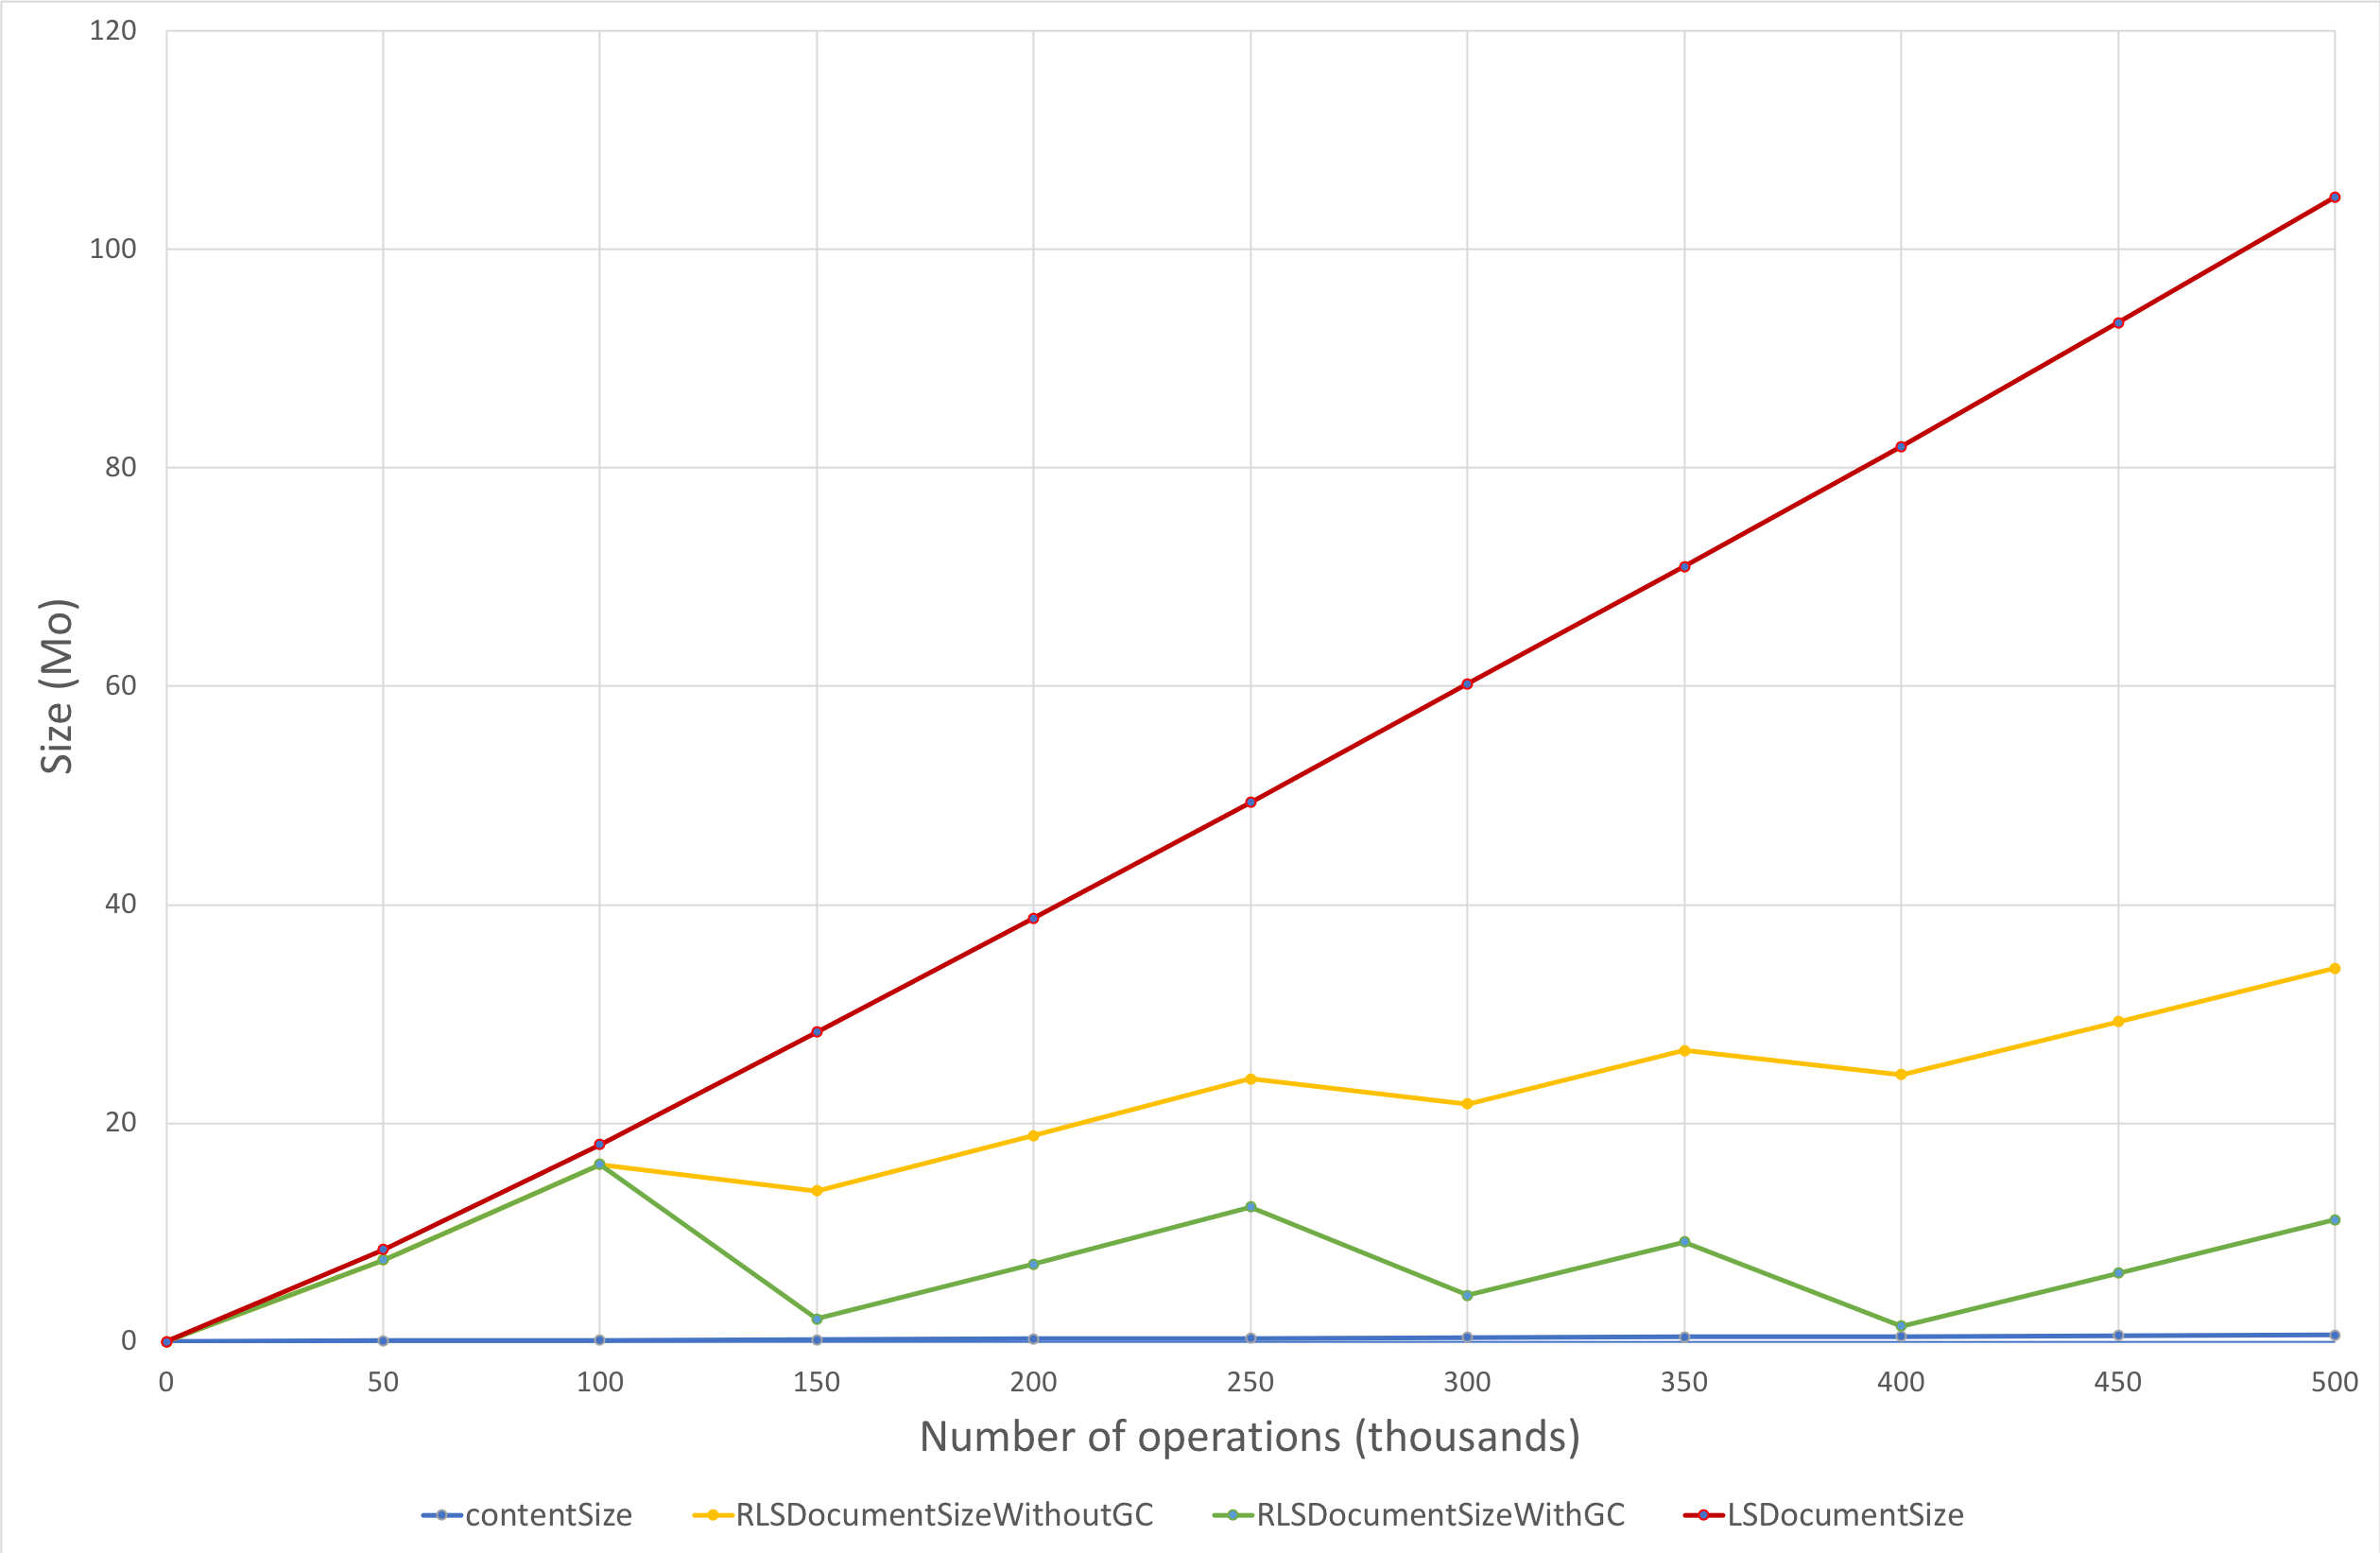
\includegraphics[width=0.8\textwidth]{img/evolution-document-size.png}
    \caption{Evolution of the size of the document}
    \label{fig:evolution-document-size}
\end{figure}

\subsection{Integration time of \emph{rename} operations}

% CPU Reference: Intel(R) Xeon(R) CPU E5-2640 v4 @ 2.40GHz

\subsection{Integration time of \emph{insert} and \emph{remove} operations}

% \subsection{Limits}

% \subsubsection{Size of concurrently generated positions}

% \mnnote{TODO: Ajouter quelques lignes sur le fait que le renommage a pour effet d'augmenter la taille des positions insérées en concurrence. Tempérer ce problème en argumentant que ce nombre de positions concurrentes devrait s'avérer faible par rapport au nombre total de positions contenues dans la séquence et qu'elles seront de toute façon réduites au cours du renommage suivant.}

% \subsubsection{Fault-tolerance}

% \begin{itemize}
%     \item The system is vulnerable to failures, as only one particular node is able to trigger renamings
%     \begin{itemize}
%         \item A failure of this node would prevent the renaming mechanism from being triggered ever again
%         \item But other nodes would still be able to continue their collaboration in such scenario
%         \item The failure of the renaming mechanism does not impede the liveness of the system
%     \end{itemize}
%     \item To address this fault-tolerance issue, can set up a consensus-based system
%     \begin{itemize}
%         \item Require nodes to perform a consensus to trigger a renaming
%         \item But consensus algorithms are expensive and not suited for dynamic systems
%         \item Can adapt the idea introduced in \cite{letia:hal-01248270}
%         \item In this paper, authors propose to divide a distributed system into two tiers:
%         the \emph{Core}, a small set of controlled and stable nodes, and the \emph{Nebula}, an uncontrolled set of nodes
%         \begin{itemize}
%             \item Only nodes from the \emph{Core} would participate in the consensus leading to a renaming
%         \end{itemize}
%         \item Provide a trade-off between the cost of performing a renaming and the resilience of the system
%     \end{itemize}
%     \item But this approach is not suited for all kind of applications
%     \item In fully distributed systems, there is no central authority to provide a set of stable nodes acting as the \emph{Core}
% \end{itemize}

\section{Renaming in a fully distributed setting}

\subsection{System Model}
\subsection{Intuition}
\subsection{Strategy to determine leading epoch in case of concurrency}
\subsection{Transitioning from a losing epoch to the leading one}
\subsection{Garbage collection}

\section{Evaluation}

\section{Discussion}

\subsection{Offloading on disk unused renaming rules}

\begin{itemize}
    \item As stated previously, nodes have to keep renamingMaps as long as another nodes may issue operations which would require to be transformed to be applied
    \item Thus nodes need to keep track of the progress of others to determine if such operations can still be issued or if it is safe to garbage collect the renaming rules
    \item In a fully distributed setting, this requirement is difficult to reach as nodes may join the collaboration, perform some operations and then disconnect
    \item Other nodes, from their point of view, are not able to determine if they disconnected temporarily or if it left definitely the collaboration
    \item However, as the disconnected nodes stopped progressing, they hold back the whole system and keep the current active nodes from garbage collecting old renaming rules
    \item To limit the impact of stale nodes on active ones, we propose that nodes offload unused renamingMaps by storing them on disk
\end{itemize}

\mnnote{TODO: Présenter une méthode pour déterminer les règles de renommage non-utilisées (conserver uniquement les règles utilisées pour traiter les $x$ dernières opérations ?)}

\subsection{Alternative strategy to determine leading epoch}
\subsection{Postponing transition between epochs in case of instability}

\begin{itemize}
    \item May reach a situation in which several nodes keep generating concurrent renaming operations on different epoch branches
    \item In such case, switching repeatedly between these concurrent branches may prove wasteful
    \item However, as long as nodes possess the required renamingMaps, they are able to rewrite operations from the other side and to integrate them into their copy, even if they are not on the latest epoch of their branch
    \begin{itemize}
        \item At the cost of an overhead per operation
    \end{itemize}
    \item Thus not moving to the new current epoch does not impede the liveness of the system
    \item Nodes can wait until one branch arise as the leading one then move to this epoch
    \item To speed up the emergence of such a branch, communications can be increased between nodes in such case to ease synchronisation
\end{itemize}

\subsection{Compressing the renaming operation}

\label{sec:optimisation-rename-op}

\mnnote{TODO: Retravailler pour y ajouter la notion d'offset. Par contre, faire remarquer qu'on a pas besoin de l'offset pour identifier de manière unique "la base" d'une position (toute la position sauf l'offset)}

\begin{itemize}
    \item Propagating the renaming operation consists in broadcasting the list of blocks on which the renaming was performed, so that other nodes are able to compute the same rewriting rules
    \item This could prove costly, as the state before renaming can be composed of many blocks, each using long positions
    \item We propose an approach to compress this operation to reduce its bandwidth consumption at the cost of additional computations to process it
    \item Despite the variable length of positions, the parts required to identify an position uniquely are fixed
    \begin{itemize}
        \item We only need the $siteId$ and the $seq$ of the last tuple of the position to do so
    \end{itemize}
    \item Instead of broadcasting the list of whole positions, the node which performs the renaming can just broadcast the list of tuples $<siteId, seq>$
    \item On reception of a compressed renaming operation, a node needs first to regenerate the list of renamed blocks to be able to apply it
    \item To achieve so, it can browse its current state looking for positions with corresponding tuples $<siteId, seq>$
    \item If some positions are missing from the state, it means that they were deleted concurrently
    \item The node can thus browse the concurrent remove operations to the renaming one to find the missing blocks
    \item Once all positions has been retrieved and the list of blocks computed, the renaming operation can be processed normally
\end{itemize}

\subsection{Operational Transformation}

\mnnote{NOTE: Ajouter une section sur OT pour expliquer que gérer les opérations concurrentes aux renommages consiste en finalité à transformer ces opérations, mais qu'on a décidé de ne pas présenter et formaliser l'approche comme étant de l'OT dans ce papier pour des raisons de simplicité ?}

\section{Related Works}

\subsection{Specification and Complexity of Collaborative Text Editing}

\mnnote{TODO: voir comment on échappe à leur spécification, en quoi on diffère. }

\subsection{LSEQ}

\mnnote{TODO: Présenter LSEQ et expliquer qu'on peut tout à fait combiner au mécanisme de renommage}

\subsection{Core and Nebula}

\mnnote{TODO: Re-présenter Core et Nebula et expliquer qu'on peut l'utiliser dans le cadre du mécanisme de renommage pour limiter les risques de renommages concurrents}

% Différences:
% - Les noeuds d'une epoch donné sont incapables de gérer les opérations provenant d'epochs précédentes
% - Les noeuds de la Nebula ont la responsabilité de transformer leurs opérations avant de pouvoir les envoyer au Core

\section{Conclusion}

\printbibliography

\end{document}
